\section{Problem 4}

\subsection{(b)}
Fitting on the first feature (CRIM) the fit() function gives me with the following weights
$$ w_{0} = 23.63506195$$ and $$w_{1} = -0.43279318$$
These values tell something about the context about the houseprices and the crimerate. The value
for a house is approximately $\$ 23.000 $ and as the crime rate rises, the value of the houses will
go down by a factore of $ -0.43279318 $

\subsection{(c)}
Fitting on alle the features the fit() function gives me with the following weights following weights.\\
\begin{align}
    \hat{\textbf{w}} &= \begin{bmatrix}
    2.05558292e+01\\
    -2.50312466e-02\\
    1.73555758e-02\\
    1.80262164e-01\\
    -1.40859425e+00\\
    7.55741436e+00\\
    -1.86729639e+00\\
    1.90656514e-02\\
    9.81506395e-01\\
    -9.99365107e-02\\
    4.17706547e-03\\
    2.56978545e-01\\
    -1.43515875e-03\\
    -2.36790752e-01\\
        \end{bmatrix}
\end{align}
\subsection{(d)}
Calculating the RMSE\\
$RMSE_{singlefeature} = 8.954859906611233$\\
$RMSE_{allfeatures} = 4.688333653627553$\\
What we can learn from the two RMSE values is, that it is possible to obtain a better fit when using more features.

\begin{figure}[H]
    \centering
    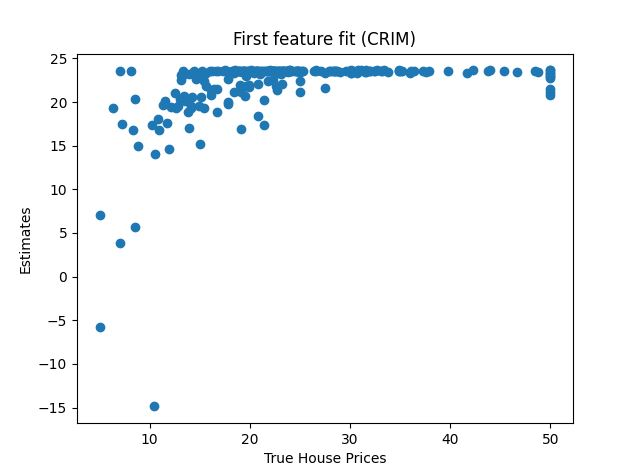
\includegraphics[width=0.9\textwidth]{Figures/Fit_one_feature.JPG}
    \caption{House prices for one feature}
\end{figure}

\begin{figure}[H]
    \centering
    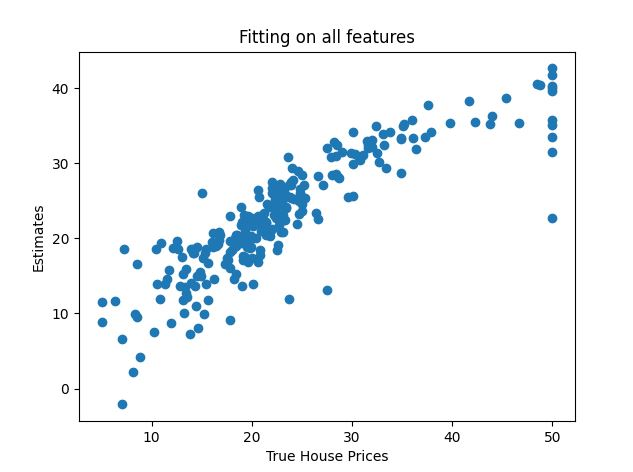
\includegraphics[width=0.9\textwidth]{Figures/fit_all_features.JPG}
    \caption{House prices for all features}
\end{figure}
For the rest of the code/results see the extended \textbf{housing\_2.py} file that has been uploaded.